\section{Results}
\label{sec:results}

\subsection{Many configurations completed, but only 156 met S1}
\label{sec:results-status}

The frozen registry contained 1,224 unique configurations with no duplicate run identifier or configuration fingerprint.  Of these, 865 (70.67\%) had completed artifacts, 19 had failed terminal states, and 340 had not been executed.  Completion did not imply exact reproduction: only 156 configurations (12.75\%) satisfied S1, while 216 (17.65\%) were S2, 122 (9.97\%) were trend-only S3, and 371 (30.31\%) were non-identifiable S4.  Thus, the S1 count was less than one fifth of the completed-artifact count.

\begin{table}[t]
\centering
\caption{Six-level evidence taxonomy in the frozen UrbanEV configuration inventory. Percentages use all 1,224 registered configurations as the denominator.}
\label{tab:status}
\small
\begin{tabular}{p{0.07\linewidth}p{0.59\linewidth}rr}
\toprule
Code & Evidence status & Count & Share \\
\midrule
S1 & Protocol and numerical result identifiable and reproduced & 156 & 12.75\% \\
S2 & Protocol broadly consistent; disclosure differences remain & 216 & 17.65\% \\
S3 & Relative trend only & 122 & 9.97\% \\
S4 & Original information cannot identify a unique configuration & 371 & 30.31\% \\
S5 & Configuration identified; execution failed & 19 & 1.55\% \\
S6 & Runnable configuration not actually completed & 340 & 27.78\% \\
\bottomrule
\end{tabular}
\end{table}


The distribution also depended on the original UrbanEV source table.  UrbanEV source Table~3 contained all 156 S1 configurations, alongside 180 S2, 94 S3, six S5, and 44 S6 configurations.  In contrast, 215 of 216 source Table~4 configurations were S4 under the frozen mapping rule.  Source Table~5 contained 156 S4 and 296 S6 configurations among 528 entries.  These patterns identify where disclosure and execution evidence was limited; they do not rank the predictive quality of the models appearing in those source tables.

\begin{figure}[t]
    \centering
    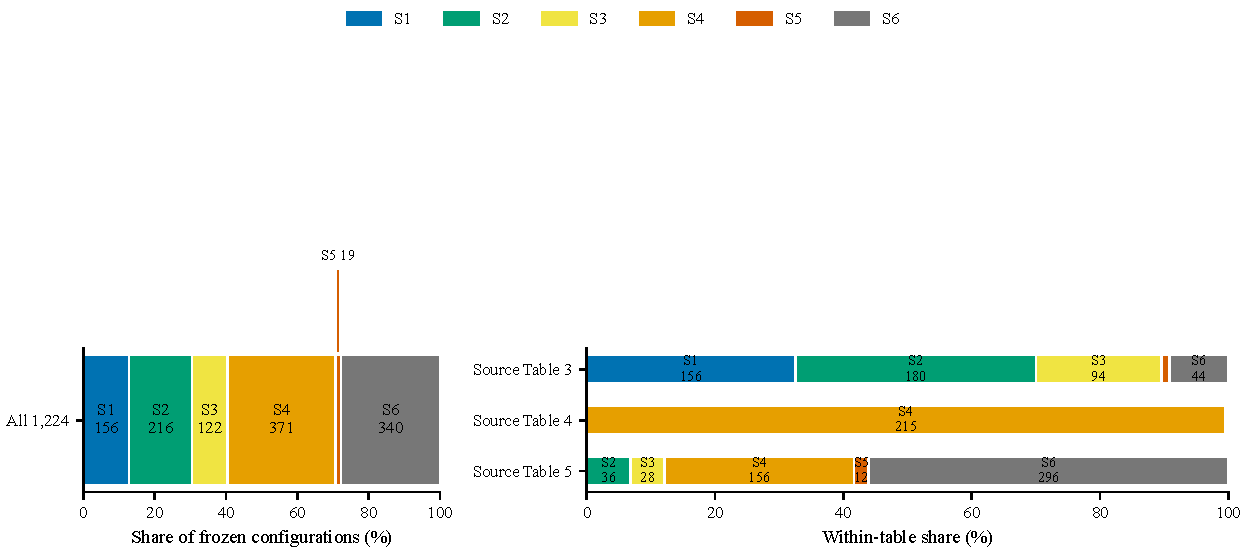
\includegraphics[width=\linewidth]{figures/fig02_configuration_status.pdf}
    \caption{Evidence status in the frozen UrbanEV inventory, overall and by source table.  Completed execution and exact reproduction are separate quantities; status counts do not measure intrinsic model quality.}
    \label{fig:configuration-status}
\end{figure}

\subsection{Fixed fusion recovered part of the oracle gain}
\label{sec:results-accuracy}

The baseline experiment completed all 72 registered runs (three models, six folds, and four horizons).  Among the evaluated single models, compact TimeXer had the lowest macro RMSE at 0.073709.  DLinear reached 0.075362, NLinear 0.075711, and GBDT-Forecaster 0.078165; CAPER's existing same-target result was 0.075507.  TimeXer was best only among the models tested under this UrbanEV protocol.

\begin{table*}[t]
\centering
\caption{Same-protocol UrbanEV accuracy results over six rolling folds and four horizons (24 equal-weight cells, seed 42). The oracle uses target-dependent expert choice and is not deployable.}
\label{tab:accuracy}
\small
\begin{tabular}{lrrrl}
\toprule
Method & Cells & Macro RMSE & Macro MAE & Evidence role \\
\midrule
GBDT-Forecaster & 24 & 0.078165 & 0.049388 & lightweight baseline \\
NLinear & 24 & 0.075711 & 0.047894 & lightweight baseline \\
CAPER & 24 & 0.075507 & 0.048480 & expert \\
DLinear & 24 & 0.075362 & 0.048041 & lightweight baseline \\
TimeXer & 24 & 0.073709 & 0.046367 & best evaluated single model \\
Global Fixed & 24 & 0.071367 & 0.044949 & strict prequential fixed fusion \\
Horizon Fixed & 24 & 0.071372 & 0.044951 & horizon-specific fixed control \\
Oracle & 24 & 0.061233 & 0.035023 & target-dependent upper-bound diagnostic \\
\bottomrule
\end{tabular}
\end{table*}


CAPER and TimeXer still made different local errors, leaving a sizeable oracle gap.  Their mean residual Pearson and Spearman correlations were 0.8422 and 0.7638, respectively.  A target-dependent oracle reduced macro RMSE to 0.061233, a 16.926\% improvement over TimeXer.  This was only an upper bound because it used the realized target to choose the expert.

Global Fixed recovered part of this oracle improvement.  Its macro RMSE was 0.071367, 3.178\% below TimeXer.  It improved all six fold means and all 24 fold--horizon cells, with horizon-level gains from 2.890\% to 3.645\%.  A paired block interval was not part of this earlier frozen accuracy protocol, so the result was not treated as passing the later router or teacher gate.  The Horizon Fixed control was nearly identical at 0.071372.  Post-hoc horizon-specific weights were therefore not needed for the fixed-fusion point result.

Predicting which expert would win was harder than the oracle gap suggested.  A rolling classifier using expert outputs and disagreement alone had mean AUC 0.5370 (range 0.5227--0.5701).  Adding 21 forecast-origin features increased LightGBM mean AUC to 0.6151.  The minimum and maximum fold AUC were 0.5660 and 0.6682, and the mean Brier score was 0.2388.  These proxy results supported running one small router experiment.  They were not evidence of better forecasts.

\subsection{The learned router produced a positive but sub-threshold gain}
\label{sec:results-router}

The hard router underperformed Global Fixed, with macro RMSE 0.072759.  Raw-probability soft routing obtained the lowest observed router RMSE, 0.070979, corresponding to a 0.543\% gain over Global Fixed.  The locked primary direct-loss MLP obtained RMSE 0.071050, a 0.443\% gain.  The better secondary point estimate did not replace that primary comparison.  The MLP won five of six folds and 18 of 24 cells, improved every horizon, and had a paired 24-hour-block gain interval of [0.275\%, 0.634\%].  It captured only 3.123\% of the oracle gap.

Although the consistency checks passed, the 0.443\% gain remained below the frozen 1\% threshold.  Gate 4 therefore failed, and router development stopped.  The result does not show that routing had no signal.  It shows that the measured gain was too small to continue under the registered rule.

\subsection{Global Fixed improved RMSE but increased latency}
\label{sec:results-latency}

The synchronous benchmark completed 90 of 90 process jobs and retained 90,000 raw timing rows.  At batch one, TimeXer required 14.067~ms median and 15.952~ms P95 end-to-end latency.  Global Fixed required 20.940~ms median and 33.123~ms P95.  Thus, the 3.178\% internal RMSE improvement came with 48.86\% higher P50 latency.  P95 latency was also higher.  NLinear and DLinear were much faster (0.674 and 1.166~ms P50) but had higher RMSE.  In this single-GPU sequential workload, Global Fixed had the lowest RMSE, but its latency was substantially higher.  Batch 8/32, model-only, throughput, environment, and portability details appear in the Supplementary Material.

\begin{table}[t]
\centering
\caption{Batch-1 end-to-end accuracy--latency trade-off on the frozen RTX 4060 Laptop GPU, FP32 single-device sequential workload.}
\label{tab:latency}
\small
\begin{tabular}{lrrrr}
\toprule
Method & RMSE & P50 ms & P95 ms & Origins/s \\
\midrule
NLinear & 0.075711 & 0.674 & 1.056 & 1483.7 \\
DLinear & 0.075362 & 1.166 & 1.763 & 857.9 \\
GBDT-Forecaster & 0.078165 & 6.242 & 7.195 & 160.2 \\
CAPER & 0.075507 & 7.934 & 10.798 & 126.0 \\
TimeXer & 0.073709 & 14.067 & 15.952 & 71.1 \\
Global Fixed CAPER+TimeXer & 0.071367 & 20.940 & 33.123 & 47.8 \\
\bottomrule
\end{tabular}
\end{table}


\begin{figure}[t]
    \centering
    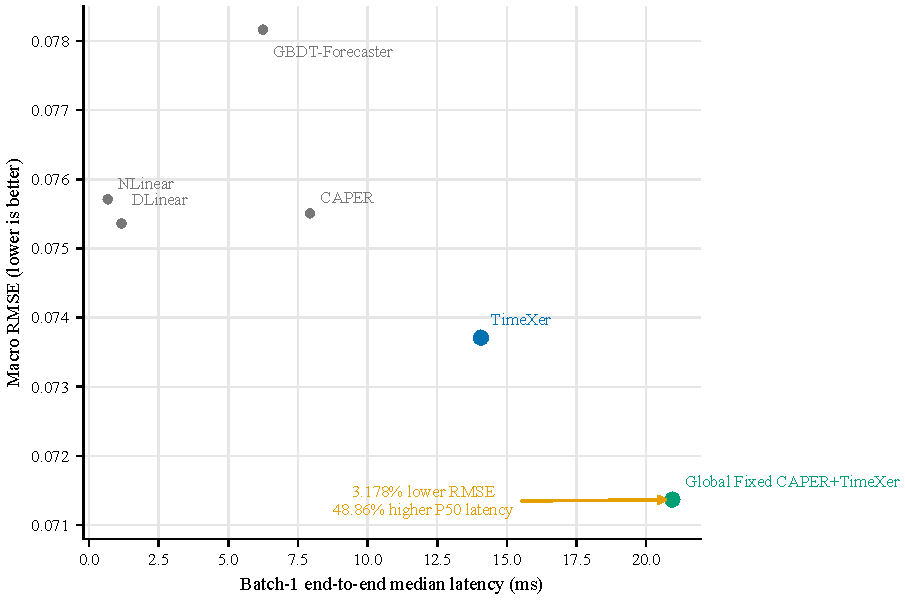
\includegraphics[width=0.82\linewidth]{figures/fig04_accuracy_latency_frontier.pdf}
    \caption{Batch-1 UrbanEV accuracy--latency frontier on the frozen RTX 4060 Laptop GPU in FP32.  The arrow from TimeXer to Global Fixed represents 3.178\% lower RMSE and 48.86\% higher median end-to-end latency.}
    \label{fig:accuracy-latency}
\end{figure}

\subsection{Chronos-2 did not qualify as the UrbanEV teacher}
\label{sec:results-chronos}

The locked Chronos-2 screen completed all 24 fold--horizon cells and 5,960 forecast origins under the zero-shot, no-future-covariate, median point-forecast setting.  Target, index, timestamp, and zone identities passed.  All inputs ended no later than the forecast origin, and a repeated sentinel prediction had maximum absolute difference zero.

Chronos-2 macro RMSE was 0.073542, compared with 0.071367 for Global Fixed, a relative gain of $-3.048\%$.  It beat the control in one of six folds and four of 24 cells.  Its RMSE deteriorated by 2.138\%--3.932\% across the four horizons.  Chronos-2 had lower secondary MAE (0.042250 versus 0.044949), but the registered decision rule used RMSE as the primary endpoint and MAE only as a secondary diagnostic.  Chronos-2 therefore failed this teacher screen, and Global Fixed remained the teacher for this project.  This result is not a general comparison between foundation forecasters and local models.

\subsection{Aligned distillation did not improve consistently over GT-only}
\label{sec:results-distillation}

The final distillation matrix contained 72 audited cells: GT-only, aligned-KD, and shuffled-teacher branches across six folds and four horizons.  Macro RMSE was 0.075568 for GT-only, 0.075478 for aligned KD, and 0.075674 for the shuffled control.  Relative to GT-only, aligned KD improved RMSE by 0.119\%, won four of six folds and 14 of 24 cells, and had a paired interval of [$-0.064\%$, 0.303\%].  It failed the frozen gain, fold, cell, and positive-lower-bound criteria, while horizon protection passed.

Aligned KD did outperform shuffled-teacher training by 0.259\%, with five of six fold wins and a paired interval of [0.151\%, 0.367\%].  This result is consistent with some sample-aligned teacher information, but it did not produce a stable improvement over the identical GT-only student.  The D1 gate failed, \texttt{distill\_v1} terminated, and neither student latency nor multi-seed or protected evaluation was run.

\subsection{Paris gains were consistent but remained below the 1\% rule}
\label{sec:results-paris}

Paris non-available-port-fraction results are reported only within the development boundary and are not compared numerically with UrbanEV.  They are not energy-demand or session-volume forecasts.  Among simple development baselines, last observation had macro RMSE 0.302630, daily lag 0.331654, and weekly lag 0.381137.  Across the 16 fold--horizon cells, the locally audited Paris CAPER adaptation obtained RMSE 0.244601 and the locally audited TimeXer adaptation 0.242542.  The strict prequential fixed teacher reduced RMSE to 0.240488; the target-dependent oracle diagnostic was 0.217661.

The teacher improved over TimeXer by 0.8469\%, won all four folds and all 16 cells, and had a paired interval of [0.6867\%, 1.0088\%].  Every bootstrap replicate selected TimeXer as the best single reference, and no horizon deteriorated.  The result was consistent, but the point estimate remained below the frozen 1\% progression rule.  Because every condition was required, the teacher gate failed.  Student training stopped, the value was not rounded into a pass, and no formal or protected access was authorized.

Formal- and protected-role target-bearing sources existed only in the procedurally isolated evidence vault.  The storage boundary was materialized and hash-audited, but analytical access count remained zero; no post-lock target value or metric from either role contributed to the Paris result or this paper.

\begin{table*}[t]
\centering
\caption{Stage-specific qualification outcomes. Gains use different frozen references and are not absolute cross-stage or cross-dataset comparisons. ``--'' for Chronos-2 means that its frozen screen did not register a paired interval, not zero uncertainty.}
\label{tab:gates}
\scriptsize
\begin{tabular}{llllll}
\toprule
Stage & Frozen reference & Gain & Paired 95\% CI & Primary point gate & Decision \\
\midrule
Router MLP & Global Fixed & +0.443\% & [0.275, 0.634]\% & 1.0\% & FAIL \\
Chronos-2 & Global Fixed & -3.048\% & -- & 1.0\% & FAIL \\
Aligned KD & GT-only student & +0.119\% & [-0.064, 0.303]\% & 1.0\% & FAIL \\
KD vs shuffled & shuffled teacher & +0.259\% & [0.151, 0.367]\% & positive control contrast & PASS SUBCHECK \\
Paris teacher & Paris TimeXer & +0.847\% & [0.687, 1.009]\% & 1.0\% & FAIL \\
\bottomrule
\end{tabular}
\end{table*}


\begin{figure}[t]
    \centering
    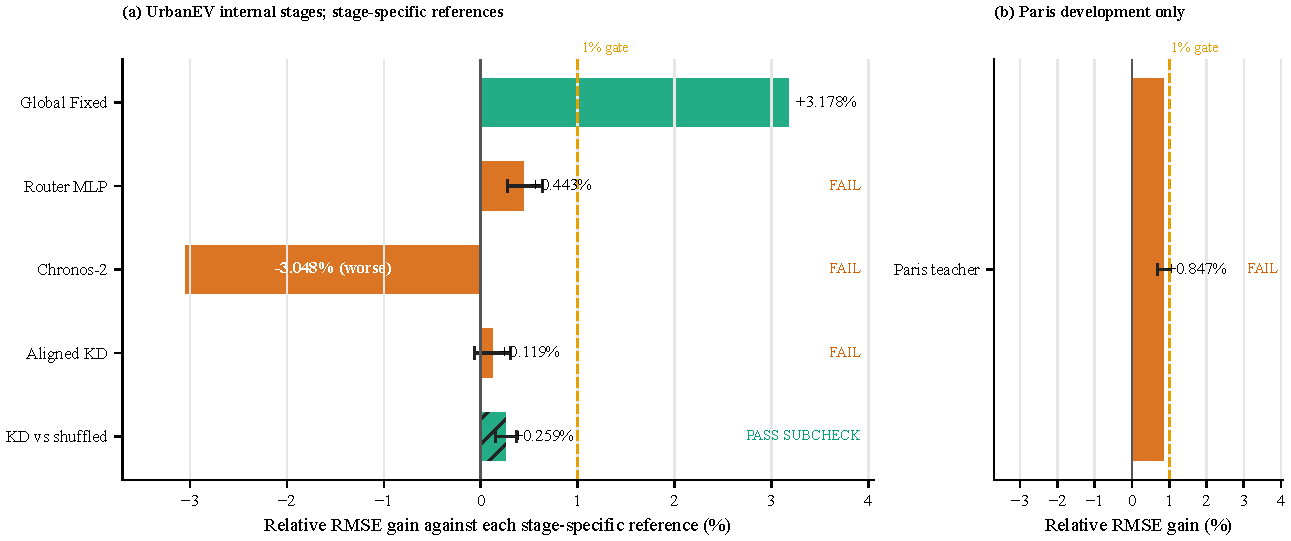
\includegraphics[width=\linewidth]{figures/fig03_stage_gain_gates.pdf}
    \caption{Stage-specific relative gains against each frozen reference.  UrbanEV and Paris use different panels, targets, and references; the plot compares gate outcomes rather than absolute RMSE.  The dashed 1\% line is the project-specific minimum effect, not a universal utility threshold.}
    \label{fig:stage-gains}
\end{figure}

\subsection{Artifact checks blocked metric access until errors were corrected}
\label{sec:results-audit-events}

The first M7-C matrix audit passed 69 of 72 cells and found that three shuffled-control mappings left the data unchanged.  Metrics remained locked.  The pipeline invalidated and reran all 24 shuffled controls instead of rerunning only the three detected cells.  The final audit passed all 72 cells before D1 metrics were computed.

\begin{table*}[t]
\centering
\caption{Fail-closed interventions performed before scientific interpretation. Repairs did not change model predictions or optimize observed metrics.}
\label{tab:audit}
\small
\begin{tabular}{>{\raggedright\arraybackslash}p{0.14\linewidth}>{\raggedright\arraybackslash}p{0.23\linewidth}>{\raggedright\arraybackslash}p{0.27\linewidth}>{\raggedright\arraybackslash}p{0.24\linewidth}}
\toprule
Event & Detection & Required action & Final state \\
\midrule
M7-C control & 3 identity mappings detected (69/72 initial audit pass) & all 24 shuffled controls rerun & 72/72 final audit PASS \\
Paris predeployment review & automated artifact audit: BLOCK & 8 blockers repaired; DEPLOY PASS & pre-run authorization only; metrics locked \\
Paris target repair & 24 runs; 10,236 masked targets restored & restore missing representation; predictions unchanged & metrics still locked \\
Paris metric unlock & 32/32 jobs closed & prediction identity audit & prediction audit PASS; metrics unlocked; teacher gate FAIL; formal/protected analysis locked; analytical access 0 \\
\bottomrule
\end{tabular}
\end{table*}


The Paris pipeline used the same fail-closed rule.  The first automated artifact audit blocked the 32 development runs because eight implementation or boundary requirements were unresolved.  After those issues were corrected, a final automated differential audit issued the internal status \texttt{DEPLOY\_PASS}.  This status authorized the development runs only; it did not indicate deployment readiness.  All 32 model jobs then closed before metric access.

A representation audit later found fill values at masked target positions in 24 of 32 artifacts, covering 10,236 entries.  The repair restored missing-value representation without retraining and left every prediction unchanged.  Metrics had still not been accessed.  A subsequent prediction audit passed 32 of 32 artifacts and then unlocked the development metrics.  These automated audits were not external human replications.

The reported negative decisions were computed only after the registered artifact checks passed.  These checks do not show that auditing improved forecast accuracy.  Throughout the Paris stage, formal and protected sources remained in vault-only storage and the analytical-access count stayed at zero.

\begin{figure}[t]
    \centering
    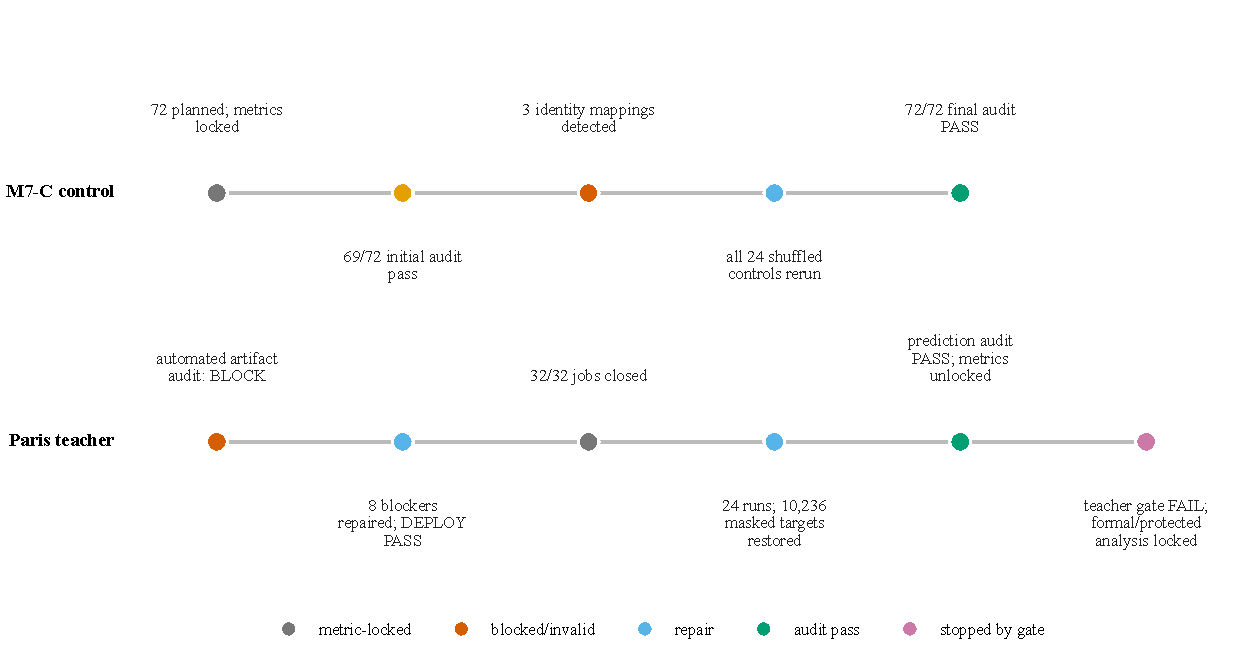
\includegraphics[width=\linewidth]{figures/fig05_audit_timeline.pdf}
    \caption{Fail-closed audit timelines.  Invalid controls and missing-target representation were corrected before metric interpretation; the corrections did not alter model predictions or authorize formal/protected analysis.}
    \label{fig:audit-timeline}
\end{figure}

The Supplementary Material links each research question to its result and supporting artifact.
